\chapter{Artificial Intelligence} % Depth 0

\section{Introduction} % Depth 1

\subsection{What is AI ?}

\begin{center}
\begin{tabular}{r|c|c}
 & \textgreen{Human} & \textgreen{Rationality} \\ 
\hline 
\textred{Thinking} & \makecell[l]{Systems that think like humans.\\\textblue{Cognitive modeling approach}} & \makecell[l]{Systems that think rationally.\\\textblue{The "Law of Tought" approach.}} \\ 
\hline 
\textred{Acting} & \makecell[l]{Systems that act like humans.\\\textblue{The Turing Test approach.}} & \makecell[l]{Systems that act rationally.\\\textblue{The rational agent approach.}} \\ 
\end{tabular} 
\end{center}

\subsubsection{Systems that think like humans} % Depth 2

\textred{The Cognitive Modeling approach} : Try to construct theories of how the human think. Synergy between computer models from Ai and experimental techniques from psychology, introspection and brain imaging.

\subsubsection{Systems that act like humans}

\textred{The Turing Test approach} : Testing if a program is able to achieve human-like performance in cognitive tasks.

\subsubsection{Systems that think rationally}

\textred{The "law of Tought" approach} : Require formal representation of problems and knowledge. Use formal reasoning systems to derive the solution.

\subsubsection{Systems that act rationally}

\textred{The rational agent approach} : \textit{standard AI model} : Agents that do the "right thing" :
\begin{itemize}
\item Achieve its goals according to what it knows
\item Perceive information from the environment
\item May use knowledge and reasoning to select actions
\item Perform actions that may change the environment
\end{itemize}

\paragraph{Value alignment problem}

Agreement between our true preference and objectives put in the machine.

\section{Intelligent Agents}

\subsection{What is an agent ?}

An agent is an entity that interacts with its environment.
\begin{itemize}
\item Perception through \textred{sensors}.
\item Actions through \textred{actuators} or effector.
\end{itemize}

\subsubsection{Rational Agents}

A \textred{rational agent} does "the right thing", i.e. the action that leads to the best outcome

\subsection{Performance of an Agent}

A \textred{performance measure} embodies the criterion for success of an agent's behavior.

For each possible percept sequence, a rational agent should select an action that is expected to maximize its performance measure, given the evidence provided by its percept sequence and whatever built-in knowledge the agent has (rationality $\neq$ perfection).

\subsubsection{Environment properties}

\begin{enumerate}
\item Fully vs. partially observable
\item Single vs. multiagent
\item Deterministic vs. stochastic
\item Episodic vs. sequential
\item Static vs. dynamic
\item Discrete vs. continuous
\item Known vs. unknown environment
\end{enumerate}

\subsection{Structure of Agents}

Agent = \textred{Architecture} + \textgreen{Program}

\begin{itemize}
\item \textred{Architecture} : operating system of the agent (computer system, specific hardware, possibly OS functions)
\item \textgreen{Program} : functions that implements the mapping from percepts to actions
\end{itemize}

\subsubsection{Basic structure of an Agent}

\begin{figure}[H]
    \centering
    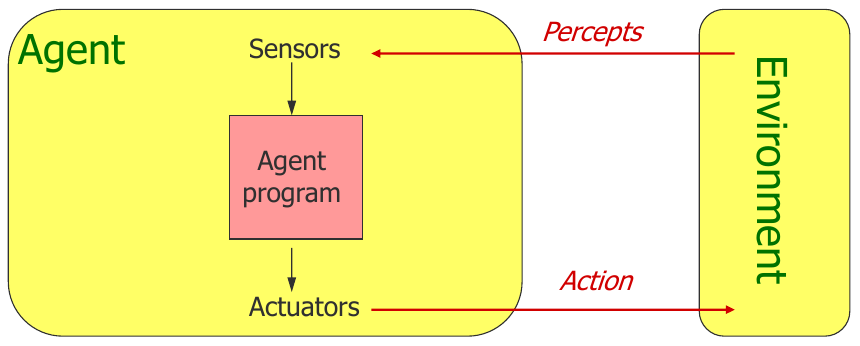
\includegraphics[width=0.6\textwidth,keepaspectratio]{basic_struct}
\end{figure}

\chapter{Problem Solving}

\section{Solving Problems by Searching}

\subsection{Search}

Process of looking for a (or the best) sequence of actions, that leads to a goal (specific state of the environment), starting from an initial state.

Hypothesis on the environment :
\begin{itemize}
\item Static
\item Discrete
\item Deterministic
\item Fully observable
\end{itemize}

\subsection{States and Actions}

\textred{States} describes distinguishable stages during problem-solving process (depend on the task and domain).

An \textred{action} transports the agent from one state to another by applying an \textred{operator} to a state.

\subsection{Formulating problems}

A \textred{problem} is defined by the items :
\begin{itemize}
\item \textgreen{States} and their representation
\item \textgreen{Initial state}
\item \textgreen{Goal stated or goal test} \textbf{Is-Goal(s)}, can be explicit (i.e."at Bucharest") or implicit (i.e. NoDirt($x$) $=$ true if $x \in \{[A,C,C],[B,C,C]\}$)
\item \textgreen{Actions} available to the agent on a given state $s$ : \textbf{Actions(s)}
\item \textgreen{Transition model} \textbf{Result(s, a)} state x action $\rightarrow$ state
\item Action \textgreen{cost function} \textbf{Action-Cost(s, a, s')} or \textbf{c(s, a, s')}
\end{itemize}

A \textred{solution} is a sequence of actions from the initial state to a goal state.
An \textred{optima solution} has the lowest path cost among all solutions.

\subsection{Searching for Solutions}

Traversal of some search space :
\begin{itemize}
\item Each node corresponds to a state
\item Root correspond to the initial state
\item Each edge corresponds to an action
\end{itemize}

\begin{itemize}
\item Expand a node $n$ by considering the possible \textbf{Actions($s$)}, where $s$ is the state in the node $n$.
\item Use \textbf{Results($s, a$)} to get the resulting states.
\item Generate new nodes with these states (called child nodes or successor nodes).
\item Attach each of these nodes to the current node as its parent.
\end{itemize}

\subsubsection{State space vs Search tree}

\begin{Parallel}[v]{0.48\textwidth}{0.48\textwidth}
\ParallelLText{\noindent
\textred{State space}\\
Possibility to infinite set of states in the world, and the associated transitions.
}
\ParallelRText{\noindent
\textred{Search tree}\\
Path between states, reaching towards the goal.\\
Possibly multiple paths from the initial state to any state.\\
Unique path back from a node to the root.
}
\ParallelPar
\end{Parallel}

\begin{minipage}{0.48\textwidth}
  \centering
  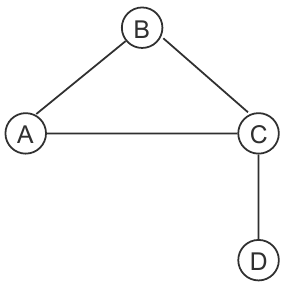
\includegraphics[width=0.3\linewidth,keepaspectratio]{state_space}
\end{minipage}
\begin{minipage}{0.48\textwidth}
  \centering
  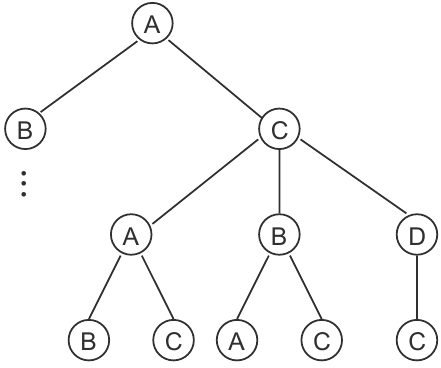
\includegraphics[width=0.4\linewidth,keepaspectratio]{search_tree}
\end{minipage}

\subsubsection{State vs. Nodes}

\textred{States} : (Representation of) a physical configuration.

\textred{Nodes} : Data structure constituting part of a search tree.

\subsubsection{Frontier}

\textred{Frontier} : set of generated nodes which have not been goal-tested (visited) and which ancestors have been goal-tested (visited).

\begin{itemize}
\item Set on unexpanded nodes
\item Separation between the visited nodes/states and the unreached nodes/states
\item Represented by a queue with operations
\item Different forms of queue will be used (priority queue, FIFO queue, LIFO queue or stack)
\end{itemize}

\subsubsection{Avoiding Repeated States}

Introduction of a look-up table containing all the visited nodes.

\subsection{Measuring performance}

\textred{Criteria}
\begin{itemize}
\item \textgreen{Completeness} : it finds a solution if one exists
\item \textgreen{Time complexity} : usually in terms of the number of nodes generated/expanded
\item \textgreen{Space complexity} : maximum number of nodes in memory
\item \textgreen{Optimality} : it finds a least cost solution ?
\end{itemize}

\textred{Problem variables}\\
Time and space complexity are measured in terms of :
\begin{itemize}
\item \textred{b} : maximum branching factor of the search tree
\item \textred{d} : depth of the least-cost solution
\item \textred{m} : maximum number of action in any path (may be infinite)
\end{itemize}

\subsection{Search Strategies}

\textred{Uninformed search} (blind search) : number of steps and path cost unknown. The agent only knows when it reaches a goal.

\textred{Informed search} (heuristic search) : agent has background information about the problem (map, costs of actions, approximation of solutions, etc.)

\subsubsection{Breadth-First Search}

\paragraph{Properties}
\begin{minipage}{0.59\textwidth}
	\begin{itemize}
	\item Complete if b is finite
	\item Time complexity : $\bigO (b^d)$
	\item Space complexity : $\bigO (b^d)$
	\item Optimal if cost = 1 per step (not optimal in general)
	\end{itemize}
\end{minipage}
\begin{minipage}{0.4\textwidth}
	\begin{figure}[H]
		\centering
    		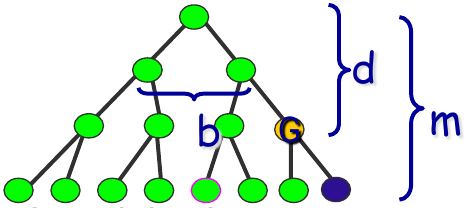
\includegraphics[width=0.6\textwidth,keepaspectratio]{properties_search}
	\end{figure}
\end{minipage}

\subsubsection{Uniform-Cost Search}

\begin{itemize}
\item The node with the lowest cost is explored first
\item Frontier is implemented as a priority queue, with f(n) = n.Path-cost
\item Equivalent to bfs if cost = 1
\item Uniform-cost search = Dijkstra algorithm
\end{itemize}

\paragraph{Properties}
\begin{itemize}
\item Complete if step cost strictly positive ($\geq \varepsilon$)
\item Time and space complexity : $\bigO (b^{1+[C^* / \varepsilon]})$, where $C^*$ is the cost of the optimal solution
\item Optimal : nodes are expanded in increasing order of g(n)
\end{itemize}

\subsubsection{Depth-first Search}

\begin{itemize}
\item Expand deepest unexpanded node
\item Frontier is implemented as a LIFO queue (stack)
\end{itemize}

\paragraph{Properties}
\begin{itemize}
\item Not complete as it can fall in infinite depth spaces
\item Time complexity : $\bigO (b^m)$
\item Space complexity : $\bigO (m*b)$
\item Not optimal
\end{itemize}

\paragraph{Depth-Limited Search}

DFS (tree-search version) with a step limit.

\subsubsection{Iterative Deepening}

Apply Depth-Limited Search with increasing depth limit. It combines the advantages of BFS and DFS methods.\\
It is the preferred uninformed search method when search space is large and depth of solution is not known.

\paragraph{Properties}
\begin{itemize}
\item Complete
\item Time complexity : $\bigO (b^d)$
\item Space complexity : $\bigO (b*d)$
\item Optimal if step cost = 1. Can be modified to explore uniform-cost tree.
\end{itemize}

\newpage
\subsubsection{Bidirectional Search}

Search simultaneously (using BFS) from goal to start and from start to goal. Stop when the two search trees intersects.

\paragraph{Properties}
\begin{itemize}
\item Complete
\item Time complexity : $\bigO (b^{d/2})$
\item Space complexity : $\bigO (b^{d/2})$
\item Optimal if cost = 1
\end{itemize}

\subsubsection{Summary}

\begin{figure}[H]
    \centering
    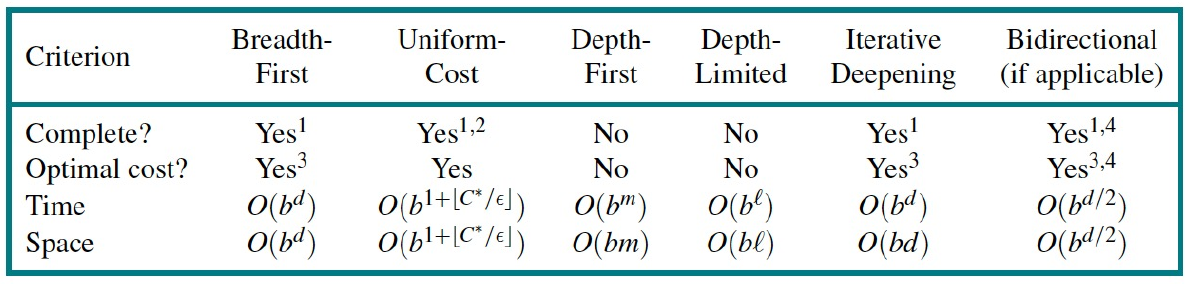
\includegraphics[width=0.7\textwidth,keepaspectratio]{search_strategies_summary}
\end{figure}

\subsection{Informed Search}

Using problem specific knowledge, find and/or deduce information about future states and future paths. Use this information to make better decisions about which paths to pursue.

A heuristic function estimates the cost of the cheapest path from node to a goal (denoted h(n)) (problem-specific).

\subsubsection{Greedy Best-First Search}

\begin{itemize}
\item Evaluate function h(n) = f(n).
\item Evaluate node that minimize h(n).
\item Expand the node that seems to be the closest to a goal.
\end{itemize}

\paragraph{Properties}
\begin{itemize}
\item Not complete as it can fall in infinite depth spaces.
\item Time complexity : $\bigO (b^m)$
\item Space complexity : $\bigO (b^m)$
\item Not optimal
\end{itemize}

\newpage
\subsubsection{A* Search}

\begin{itemize}
\item Combines greedy and uniform-cost search
\item Choose the (estimated) cheapest path through the current node
	\begin{itemize}
	\item \textgreen{f(n)} = g(n) + h(n) = path cost + estimated cost to the goal.
	\item g(n) : \textgreen{exact cost} from initial state to node $n$
	\item h(n) : \textgreen{estimated cost} from node $n$ to a goal
	\end{itemize}
\item A* can use the tree or graph search version of the generic BFS algorithm
\item h(n) is \textred{admissible} if it never overestimated the cost to reach a goal. Consequences :
	\begin{itemize}
	\item h(n) is optimistic
	\item f(n) never overestimates the cost of a solution through node $n$
	\item h(n) = 0 if $n$ is a goal
	\end{itemize}
\end{itemize}

\paragraph{Properties}
\begin{itemize}
\item Complete
\item Time complexity : $\bigO (b^d)$
\item Space complexity : $\bigO (b^d)$ (keeps all generated nodes in memory
\item Optimal and optimally efficient (if $h(n)$ consistent (Graph search) / if $h(n)$ is admissible (Tree search))
\end{itemize}

\paragraph{A* is Optimal : Proof}

A* (using \textgreen{Tree Search}) is optimal if h(n) is admissible.

\textred{Proof} :
\begin{itemize}
\item A solution is a path from the initial state to a goal state
\item Let $C^*$ be the lowest path cost among all solutions
\item We must show that A* will not return a suboptimal path to a goal
\end{itemize}
\textred{Part 1} :
\begin{itemize}
\item Let $G$ be a goal node in the frontier, but in a suboptimal path
\item Its path cost $g(G)=C$ is not the lowest one ($C>C^*$)
\item $f(G) = g(G) + h(G)$
	\begin{itemize}
	\item $h(G) = 0$ because $G$ is a goal node and $h$ is admissible
	\item $f(G) = g(G) = C > C^*$
	\item[$\rightarrow$] \textred{$f(G) > C^*$}
	\end{itemize}
\end{itemize}
\textred{Part 2} :
\begin{itemize}
\item Let $n$ be a node in the frontier, with $n$ the path to the optimal solution (cost $C^*$)
\item $f(n) = g(n) + h(n)$
\item[$\rightarrow$] \textred{$f(n) \leq C^*$} because $h$ is admissible
\end{itemize}
\textred{Part 3} :
\begin{itemize}
\item $f(n) \leq C^* < f(G)$
\item[$\rightarrow$] Node G will never be selected
\end{itemize}
\textred{Consequence} : A* expands no node with $f(n) > C^*$

\subsubsection{Consistent Heuristics}

A heuristic function is \textred{consistent} if for every node \textred{$n$} and successor \textred{$n'$} obtained with action \textred{a} :


\begin{minipage}{0.59\textwidth}
	\begin{itemize}
	\item Estimated cost of reaching goal from \textred{$n$} is no greater than cost of getting to \textred{$n'$} plus estimated cost of reaching goal from \textred{$n'$}
	\item $h(n) \leq c(n, a, n') + h(n')$
	\end{itemize}
\end{minipage}
\begin{minipage}{0.4\textwidth}
	\begin{figure}[H]
		\centering
		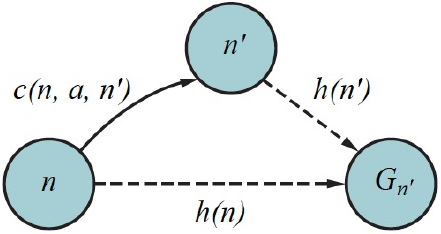
\includegraphics[width=0.7\textwidth,keepaspectratio]{triangle_inequality}
	\end{figure}
\end{minipage}

If a heuristic if consistent, then it is also admissible.\\
If $h(n)$ is consistent, then $f(n)$ along any path is non decreasing.

\paragraph{Satisficing search}
Reduce the number of visited nodes by accepting suboptimal solutions, but "good enough".

\paragraph{Memory-Bounded Heuristic Search}
Try to reduce memory needs by taking advantage of heuristic to improve performance (Iterative-deepening A* (IDA*), Recursive BFS (RBFS), Simple Memory-Bounded A* (SMA*))

\subsubsection{Iterative Deepening A*}

DFS but expand only nodes with f-cost less than or equal to smallest f-cost of non expanded nodes at last iteration. Non efficient when the number of different f-cost is high.

\paragraph{Properties}
\begin{itemize}
\item Complete
\item Time complexity : still exponential
\item Space complexity : linear
\item Optimal, optimally efficient ($h(n)$ consistent) and optimal in the absence of monotonicity
\end{itemize}

\subsubsection{Recursive Best-First Search}

DFS combined with best alternative :
\begin{itemize}
\item Keeps track of options along fringe
\item As soon as current DF exploration becomes more expensive of best fringe option, back up to fringe, but update node costs along the way.
\end{itemize}

\paragraph{Properties}
\begin{itemize}
\item Time complexity : hard to describe : efficiency is heavily dependent on quality of $h(n)$, same states may be explored many times
\item Space complexity : $\bigO (bd)$ space complexity if $h(n)$ is admissible
\end{itemize}

\newpage
\subsubsection{Simple Memory-Bounded A*}

Use all available memory with new expanded nodes. If new node does not fit : remove stored node with worse f-value, then propagate f-value of removed node to parent. It will regenerate a subtree only when it is needed (the path through the subtree is unknown, but cost is known)

\paragraph{Properties}
\begin{itemize}
\item Complete if there is enough memory for the shortest solution path
\item Time complexity : same as A* if enough memory to store the three
\item Space complexity : use available memory
\item Optimal if enough memory to store the best solution path
\end{itemize}

\subsubsection{Comparing two heuristics}

\begin{itemize}
\item Compare the total number of generated nodes \textgreen{$N$}
\item Compare the search trees : \textred{effective branching factor} : \textgreen{$b*$}
\end{itemize}

Choose the most dominant heuristic (most informed)

\begin{itemize}
\item Creating $h(n)$ by simplifying the problem by reducing restrictions on actions (\textred{relaxed problem}).
\item If multiple heuristics available : $h(n) = max{h_1(n), h_2(n), ..., h_n(n)}$
\item Performance of informed search depends on the quality of the heuristics.
\end{itemize}

\section{Search in complex environments (Local Search)}

Local search does not keep track of paths : it keeps track of the current solution (current state).

Advantages :
\begin{itemize}
\item Use a small amount of memory
\item They can find reasonable solutions in infinite search queries
\item Reasonable $\neq$ optimal
\end{itemize}

It's an incomplete method based on iteratively improving the current solution. The next solution is found in the \textred{neighborhood} of the current solution. Typically modify the value of a variable in an assignment at each step. The new solution is close to the previous one in the space of assignment.

An \textred{objective function} is a function with vector inputs and scalar inputs. Search through candidate input vectors in order to \textit{minimize} or \textit{maximize} objective function

\textred{Search space} : The set of feasible input vectors

\textred{Connected neighborhood} : from each solution, there is a path to an optimal solution.\\
Advantages :
\begin{itemize}
\item No need of a restarting strategy to reach optimal solutions
\item Required for convergence property of metaheuristics
\end{itemize}

Feasibility with optimality :
\begin{itemize}
\item Maintain feasibility at all times, explore only feasible solutions.\\
Or
\item Do not maintain feasibility at all time; relax a subset of the constraints. Explore a larger search space, drive the search to high quality and feasible solutions.
\end{itemize}

\subsection{Heuristics and metaheuristics}

\begin{Parallel}[v]{0.48\textwidth}{0.46\textwidth}
\ParallelLText{
	\textred{Heuristics}
	\begin{itemize}
	\item Choose the next solution in the neighborhood
	\item Based on local information : the current solution and its neighborhood
	\item Drive the search towards \textgreen{local optimum}
	\item Memoryless
	\end{itemize}
}
\ParallelRText{
	\textred{Metaheuristics}
	\begin{itemize}
	\item Collect information on the execution sequence(s)
	\item Aim at escaping from local optima
	\item Drive the search toward \textgreen{global optimality}
	\item Typically include memory or learning 
	\end{itemize}
}
\ParallelPar
\end{Parallel}

\subsubsection{Systematic heuristics}
Exploration (possibly partial) of the neighborhood to determine the next solution

\subsection{Hill Climbing}
Shape of state greatly influences hill climbing. Local maxima are the Achilles heel. Hill climbing never makes downhill moves (cannot escape local maxima)

\subsubsection{Random walks}
Randomized heuristics. Select an element of the neighborhood randomly. Decide whether to accept it as the next solution.

\subsection[Simulated Annealing]{Simulated Annealing\footnote{\textgreen{Annealing} is the process of heating metal and letting it cool slowly to lock in the stable locations of the molecules.}}

\begin{itemize}
\item Always move uphill if possible
\item Sometimes go downhill
\item Optimality guaranteed with slow annealing schedule
\item No need for smooth search space
\item Applicable to discrete search space
\end{itemize}

\subsection{Metropolis Step}
\textit{current $:=$ next} only with probability $e^{\Delta E/T}$ 
\begin{itemize}
\item $\Delta E$ < 0
\item $|\Delta E|$ high $\rightarrow$ probability small
\item$T$ high $\rightarrow$ probability high
\end{itemize}

The rate at which $T$ is decreased and the amount it is decreased is prescribed by an \textgreen{schedule}.\\
Bltzmann distribution : if the schedule lowers $T$ to $0$ slowly enough, then :
\begin{itemize}
\item All the probability concentrated on the global maxima
\item Global maxima will be found with probability approaching $1$
\end{itemize}

\subsection{Local Beam Search}
Keep $k$ states in memory : at each step, generate all the successors of all $k$ states. Stop if one is a goal. Otherwise select the $k$ best solutions from the complete list.

\newpage
\subsection{Genetic Algorithms (GAs)}

Randomized search algorithms based on the theory of evolution.
\begin{itemize}
\item Start with $k$ initial guesses :
	\begin{itemize}
	\item They form a \textgreen{population}
	\item Each \textgreen{individual} from the population is a fixed-length string (gene)
	\item Each individual's \textgreen{fitness} (score) is evaluated
	\end{itemize}
\item Produce a next generation by \textgreen{reproduction} between individuals from current population
\end{itemize}

GA work best if the representation stores related pieces of the puzzle in neighboring cells of string. Crossover s not applicable to all problems.

\subsection{Tabu search Metaheuristics}
Select the best neighbor that has not yet been visited. Difficult to keep track of all the visited nodes. Short-term memory : only maintain a suffix of the sequence of visited nodes.
\begin{itemize}
\item \textgreen{Transition abstraction} : represent the suffix by an abstraction (problem dependent)
\item \textgreen{Aspiration} : override the tabu status if the move improves the best solution found so far
\end{itemize}

\subsection{Intensification vs. Diversification}

\begin{Parallel}[v]{0.48\textwidth}{0.48\textwidth}
\ParallelLText{
\textred{Intensification}
	\begin{itemize}
	\item Goal : increase search around promising areas
	\item Risk : premature convergence (local minima)
	\item Mean : favor good solutions
	\end{itemize}
}
\ParallelRText{
	\textred{Diversification}
	\begin{itemize}
	\item Goal : explore new areas
	\item Risk : convergence to optimality may be too long
	\item Mean : probabilistic choice of solutions
	\end{itemize}
}
\ParallelPar
\end{Parallel}

\subsection{Other Local Search Approaches}

\textred{Variable Neighborhood Search} : Sequence of (increasing size) neighborhood\\
\textred{Guided Local Search} : Use a sequence of objective functions to drive away from local optima\\
\textred{Adaptive Local Search} : The heuristics/metaheuristics are dynamically adapted during the search\\
\textred{Ant Colony Optimization} : The selection function is updated\\
\textred{Statistic Local Search} : Another name for Local Search, stressing the stochastic aspect of the search

\section{Constraint Satisfaction Problems (CSP)}

\subsection{Constraint Satisfaction Problem}

\subsubsection{What is CSP ?}

\begin{itemize}
\item A set of \textred{variables} defined over domains
\item A set of \textred{constraints} over the variables
\end{itemize}

\subsubsection{What is a solution ?}

\begin{itemize}
\item A \textred{solution} is a consistent \textred{assignment} of values to the variables
\item \textred{Consistent} assignment : does not violate any constraint
\end{itemize}

\subsubsection{Types of CSP}

\begin{itemize}
\item Discrete and finite domains (combinatorial problems, boolean CSP)
\item Discrete and infinite domains (scheduling, linear/non-linear constraints)
\item Continuous (and infinite) domains (linear programming, continuous CSP methods)
\end{itemize}

\subsubsection{Types of constraint}

\begin{itemize}
\item Unary constraints (SA $\neq$ green)
\item Binary constraints (SA $\neq$ WA, $X+Y \leq 12$, ...)
\item Higher-order constraints ($X+5Y-3Z \leq 8$, Alldiff($V,W,X,Y,Z$), ...) can be transformed in binary constraints (with additional variables
\end{itemize}

\subsection{Constraint Propagation}

\subsubsection{CSP as a search problems}

\begin{itemize}
\item \textred{Initial state} : empty assignment
\item \textred{Successor function} : assign a value to an unassigned variable
\item \textred{Goal test} : is the current assignment complete ?
\item \textred{Path cost} : constant value per step (the path is irrelevant)
\end{itemize}

\subsubsection{Forward checking}

When $X$ is assigned a value $V$ :
\begin{itemize}
\item Look at each unassigned variable $Y$ connected to $X$ (through a binary constraint $c(X,Y)$)
\item Remove from $Y$'s domain any value inconsistent with the value chosen for $X$
\end{itemize}

\subsubsection{Objectives of constraint propagation}

\begin{itemize}
\item Reduce the search space
\item Find an equivalent CSP to the original one with \textit{\textred{smaller domains}} of variables
\end{itemize}

\subsubsection{Techniques}

\begin{itemize}
\item Consider the constraints locally
\item Arc consistency : consider constraints between $2$ variables
\item Path consistency : consider constraints between $n$ variables
\end{itemize}

\paragraph{Arc consistency}

A constraint $c(X, Y)$ is arc consistent if for every value a in the domain $X$, there is a value $b$ in the domain of $Y$ such that $c(a,b)$ is satisfied.\\
Objective : make all constraints arc consistent.

\paragraph{Bound consistency}

Weaker form of arc consistency. Only consider the bounds of the domains, never remove values in the middle of the domain; only move the bounds. Efficient propagation, less pruning.

\subsection{Backtracking Search for CSPs}

\subsubsection{Incremental formulation}

\begin{itemize}
\item Search tree : depth $n$ (number of variables)
\item BS is applicable
\item Number of states = $\bigO (d^n)$ with $n$ = number of variables, $d$ = size of the domain (discrete finite domains)
\item NP-complete problems (3SAT) 
\end{itemize}

CSP search algorithms should only consider a single variable at each node.

\subsubsection{General algorithm for any CSP}

\begin{itemize}
\item No initial state, successor function, goal test.
\item The same for each CSP
\end{itemize}

\subsubsection{Minimum remaining value (MRV) heuristics}

\begin{itemize}
\item Choose the variable with the fewest legal values
\item Most constrained variable
\item First-fail heuristics
\end{itemize}

\subsubsection{Degree heuristic}

\begin{itemize}
\item Variable involved in the largest number of constraints
\item Reducing the branching factor of substree
\item Usually used as tie-breaker of MRV
\end{itemize}

\subsection{Local search for CSPs}

\subsubsection{Complete state formulation}

\begin{itemize}
\item \textred{Initial state} : a value to every variable
\item \textred{Successor function} : change the value of one variable
\item \textred{Goal test} : is the current assignment consistent ?
\item \textred{Path cost} : constant value per step
\end{itemize}

\subsubsection{Min-Conflict Algorithm}
\begin{itemize}
\item Specialized version of Hill Climbing
\item Choosing a neighbor with a variable and new value with the min number of conflicts
\end{itemize}

\subsection{Structure of the problems}

\begin{itemize}
\item Independent subproblems (partition of variables and constraints, forming $k$ different CSPs)
\item Can be solved separately
\item Global solution is the union of the different solutions
\item Complexity $\bigO (d^{n/k} k)$
\end{itemize}

\subsubsection{Tree-structure Subproblems}

\begin{itemize}
\item Any $2$ variables are connected by at most one path.
\item Can be solved by in $\bigO (n*d^2)$
\item Few CSP are tree structured
\item How to reduce a CSP to a tree-structured CSP ? Remove nodes / collapse nodes
\end{itemize}

\begin{figure}[H]
    \centering
    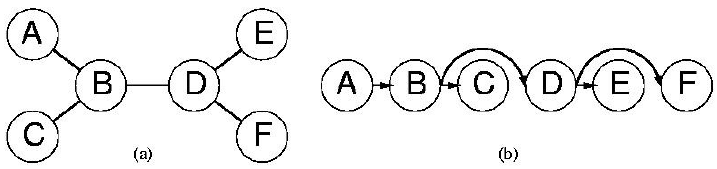
\includegraphics[width=0.6\textwidth,keepaspectratio]{tree-structure}
\end{figure}

\paragraph{Removing nodes}


\begin{minipage}{0.58\textwidth}
	\begin{itemize}
	\item Determine the cycle cutset $S$ (size $c$)
	\item Solve the reduced problem for each consistent assignment of the cutset
	\item Complexity $\bigO (d^c (n-c)d^2)$
	\end{itemize}
\end{minipage}
\begin{minipage}{0.4\textwidth}
	\begin{figure}[H]
		\centering
		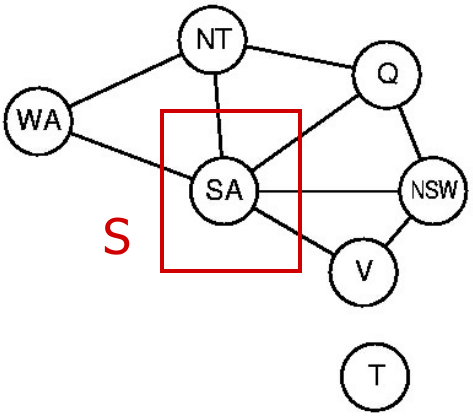
\includegraphics[width=0.4\textwidth,keepaspectratio]{removing_nodes}
	\end{figure}
\end{minipage}


\paragraph{Grouping nodes}

\begin{minipage}{0.58\textwidth}
	\begin{itemize}
	\item Tree decomposition of the constraint graph into a set of connected subproblems
	\item Each variable appears in at least one subproblem
	\item Two variables connected by a constraint must appear together in at least one subproblem
	\item If a variable appears in $2$ subproblems, it must appear in all subproblems in the path connected these subproblems.
	\end{itemize}
\end{minipage}
\begin{minipage}{0.4\textwidth}
	\begin{figure}[H]
		\centering
		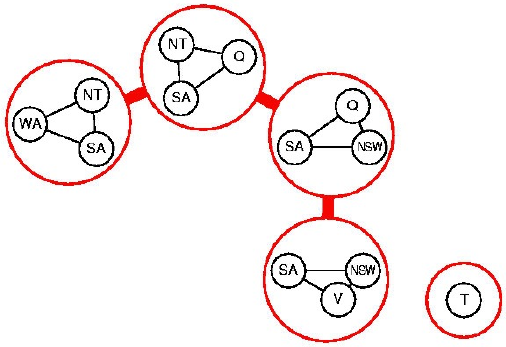
\includegraphics[width=0.6\textwidth,keepaspectratio]{grouping_nodes}
	\end{figure}
\end{minipage}

\section{Adversarial Search \& Games}

\subsection{Types of games}

\begin{center}
\begin{tabular}{l|c|c}
 & Deterministic & Chance \\ 
\hline 
Perfect information & Chess, Checkers, Go, Othello & Backgammon, Monopoly \\ 
\hline 
Imperfect information &  & Bridge, Poker, Scrabble, Nuclear war \\ 
\end{tabular} 
\end{center}

Problems involving :
\begin{itemize}
\item Multiple agents
\item Competitive environments
\item Agents have conflicting goals
\end{itemize}

\subsection{Defining a Game}

A game can be defined by the following properties :
\begin{itemize}
\item The \textred{initial state} $S_0$ (the board position)
\item To-Move($s$) : the player to play in state $s$
\item Actions($s$) : the set of legal moves in state $s$
\item Result($s, a$) : the \textred{transition model}; state resulting from taking action $a$ in state $s$
\item Is-Terminal($s$) : a \textred{terminal test} on states
\item Utility($s, a$) : a \textred{utility function} on terminal states
\end{itemize}

\newpage
\subsection{Game Tree}

Initial states and Action($s$) and Results($s,a$) define the state space search and a \textred{game tree}.\\
Two players : \textit{MAX} and \textit{MIN}.

\subsubsection{Minimax Strategy}

\textred{Minimax}($s$) =
\begin{itemize}
\item Utility($s,$ MAX) if $s$ is a terminal state
\item max$_{a \in \textit{Actions}(s)}$ Minimax(Result($s, a$) if To-Move($s$) = MAX
\item min$_{a \in \textit{Actions}(s)}$ Minimax(Result($s, a$) if To-Move($s$) = MIN
\end{itemize} 

\paragraph{Optimal strategy}
\begin{itemize}
\item Perfect play for deterministic games
\item Leads to outcomes at least as good as any other strategy when playing an infallible opponent
\item if MIN does not play optimally, MAX will do even better
\end{itemize}

\paragraph{Algorithm}

\begin{enumerate}
\item Generate the game tree to the terminal states
\item Apply the utility function to all terminal states
\item Determine the utility of the successor nodes of the terminal states
\item Treat one layer at a time, applying Min or Max
\item The value at the top of the tree determines the best move
\end{enumerate}

\paragraph{Properties}

\begin{itemize}
\item Complete (if tree is finite)
\item Time complexity : $\bigO (b^m)$
\item Space complexity : $\bigO (bm)$ where $b$ is the branching factor and $m$ the maximum depth of the search tree
\end{itemize}

\paragraph{Pruning}

\begin{itemize}
\item Discards parts of the search tree (guaranteed not to contain good moves)
\item Same best result than Minimax
\item Substantial time and space savings (cuts the exponent in half but still exponential)
\end{itemize}

\subsubsection{Alpha-Beta}

\begin{itemize}
\item Generate the tree depth-first, left-to-right
\item Propagate final values of nodes as initial estimates for their parent nodes
\end{itemize}
\begin{minipage}{0.4\textwidth}
	\begin{figure}[H]
		\centering
		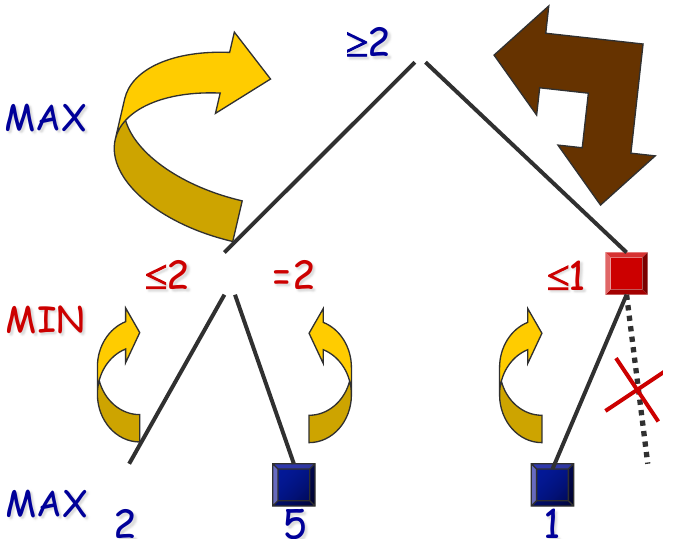
\includegraphics[width=0.6\textwidth,keepaspectratio]{alpha-beta}
	\end{figure}
\end{minipage}
\begin{minipage}{0.58\textwidth}
	\begin{enumerate}
	\item The \textred{MIN}-value (1) is already smaller than the MAX-value of the parent (2)
	\item The \textred{MIN}-value can only decrease further
	\item The \textblue{MAX}-value is only allowed to increase
		\begin{enumerate}
		\item[$\rightarrow$] No point in computing further below this node
		\end{enumerate}
	\end{enumerate}
\end{minipage}

\paragraph{Terminology}

\begin{minipage}{0.58\textwidth}
	The (temporary) values at \stackanchor[8pt]{\textblue{MAX}}{\textred{MIN}}-nodes are \stackanchor[8pt]{\textblue{ALPHA}}{\textred{BETA}}-values
\end{minipage}
\begin{minipage}{0.4\textwidth}
	\begin{figure}[H]
		\centering
		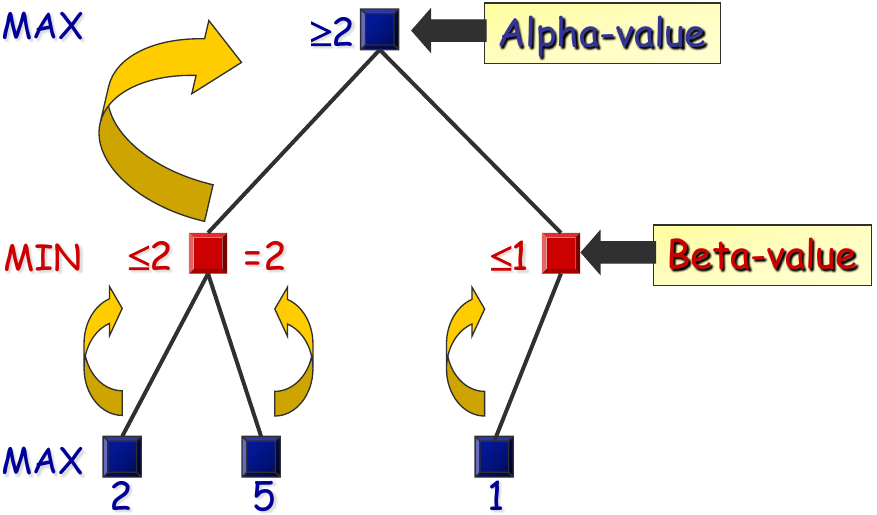
\includegraphics[width=0.8\textwidth,keepaspectratio]{alpha-beta_terminology}
	\end{figure}
\end{minipage}

\paragraph{Pruning}

\begin{itemize}
\item \stackanchor[8pt]{\textblue{$\alpha$}}{\textred{$\beta$}} : the value of the best \stackanchor[8pt]{\textblue{highest}}{\textred{lowest}} choice found so far at any choice point along the path for \stackanchor[8pt]{\textblue{MAX}}{\textred{MIN}}
\item Order of considering successors matters : if possible, consider best successors first
\end{itemize}

\paragraph{Properties}

\begin{itemize}
\item Pruning \textred{does not} affect final result
\item If successors are ideally visited, time complexity is $\bigO (b^{m/2})$ where $b$ is the branching factor and $m$ the maximum depth of the search tree (can look twice as far as minimax)
\item If successors are visited randomly, time complexity is $\bigO (b^{3m/4})$
\item Use heuristic ordering function to optimize the choice
\end{itemize}

\subsubsection{Game Tree versus Graph}

\begin{itemize}
\item Possible to memorized visited states
\item Store the evaluation of these states
\item Called \textred{transposition} tables (reached list)
\item Impractical to store all the states
\end{itemize}

Complete search is \textit{impractical for most games}. Alternative :
\begin{itemize}
\item Search only part of the tree
\item Use a \textred{heuristics}-based evaluation function to estimate the expected utility of the game from a given position
\end{itemize}

\subsubsection{Evaluation Function}

\begin{itemize}
\item \textred{H-Minimax}($s, d$) =
	\begin{itemize}
	\item Eval($s$) if Is-cutoff($s, d$)
	\item max$_{a \in \textit{Actions}(s)}$H-Minimax(Result($s, a$), $d+1$) if To-Move($s$) = MAX
	\item min$_{a \in \textit{Actions}(s)}$H-Minimax(Result($s, a$), $d+1$) if To-Move($s$) = MIN
	\end{itemize}
\item Must be consistent with the utility function
\item Tradeoff between accuracy and time cost
\item Should reflect the actual chances of winning
\item Weighted linear functions are frequently used
\end{itemize}

\subsubsection{The horizon effect}

Because of the depth-bound, we prefer to delay disasters although we don't prevent-them.
\begin{figure}[H]
	\centering
	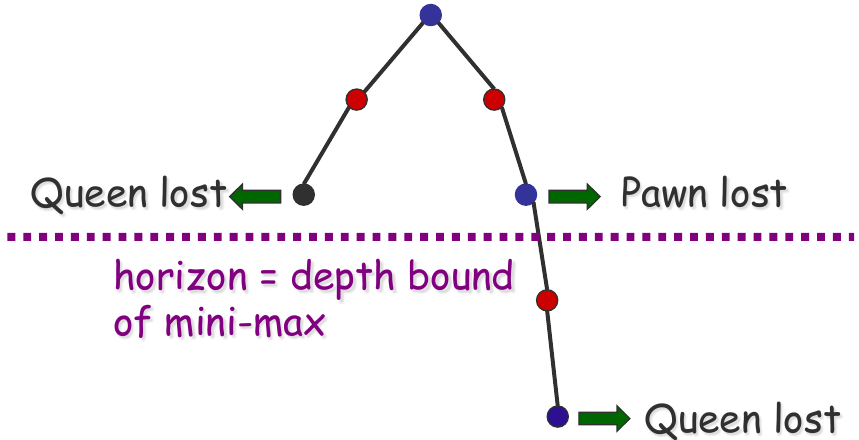
\includegraphics[width=0.4\textwidth,keepaspectratio]{horizon-effect}
\end{figure}

\subsubsection{Search strategy}

\begin{itemize}
\item Basic strategy : depth-limited
\item Beam search : only consider the $n$ best moves
\item Iterative deepening :
	\begin{itemize}
	\item Answer is refined progressively
	\item Ensure an answer within a time limit (real-time decision)
	\item Doesn't take advantage of knowledge about the problem
	\end{itemize}
\end{itemize}

\subsubsection{Search vs. lookup}

Many game-playing programs use table lookup rather than search for the opening and ending of games. End game can be completely solved by the computer.

\subsubsection{Monte Carlo tree search}

\begin{itemize}
\item Utility function estimated as the average utility (e.g. win percentage) over simulations (playout) of complete games
\item Playout with random legal moves by both players
\end{itemize}

Maintain a search tree, growing it at each iteration :
\begin{itemize}
\item Selection : starting from the root, go to a leaf using a selection strategy (focus on relevant parts)
\item Expansion : add one new child to the node
\item Simulation : playout (without recording the moves)
\item Back-propagation : update all the parents in the search tree
\end{itemize}

\chapter{Knowledge, Reasoning \& Planning}

\section{Logical Agents and Propositional Logic}

\subsection{Knowledge Based Agents}

\begin{minipage}{0.58\textwidth}
	\begin{itemize}
	\item Knowledge \textred{representation}
	\item \textred{Reasoning} with knowledge : determining which action to take
	\item \textred{Logic} deals with both of these :
		\begin{itemize}
		\item Classic logic : definite knowledge (knowledge that is true or false in the world)
		\item Other logic : uncertain knowledge
		\end{itemize}
	\end{itemize}
\end{minipage}
\begin{minipage}{0.4\textwidth}
	\begin{figure}[H]
		\centering
		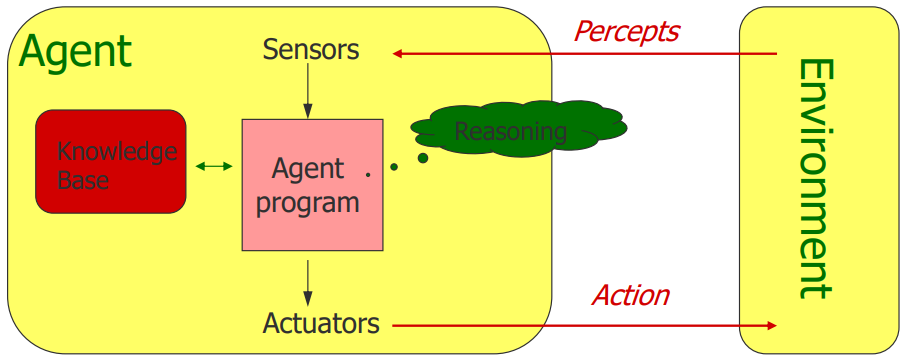
\includegraphics[width=0.9\textwidth]{knowledge_based_agents}
	\end{figure}
\end{minipage}

\begin{itemize}
\item The \textred{knowledge base} (KB) is the central component (a set of \textred{sentences} representing assertions about the world, sentences are represented with  a \textgreen{knowledge representation language})
\item Two operations on KBs : \textgreen{Tell} and \textgreen{Ask}. Both may involve \textred{inferencing}, deriving new sentences from old.
\item Agent may have initial information in KB (background knowledge)
\end{itemize}

\subsubsection{Declarative vs. Procedural}

\begin{center}
\textred{Knowledge representation}
\end{center}
\begin{Parallel}[v]{0.48\textwidth}{0.48\textwidth}
\ParallelLText{
\textred{Declarative} approach
\begin{itemize}
\item Design representation language making it easy to express knowledge
\item Simplify construction of solutions
\end{itemize}
}
\ParallelRText{
\textred{Procedural} approach
\begin{itemize}
\item Knowledge is embodied in the algorithms and program code itself
\item Potentially more efficient, but more difficult to develop solutions
\end{itemize}
}
\ParallelPar
\end{Parallel}

\subsection{Logic}

A logic consists of \textred{syntax} and \textred{semantics}
\begin{itemize}
\item \textred{Syntax} defines well formed sentences
\item \textred{Semantics} defines "meaning" of sentences. in logic, defines the \textgreen{truth} of each sentence with respect to each \textgreen{possible word (interpretation)}
\end{itemize}

\subsubsection{Interpretation and Models}

An \textred{interpretation} is a mathematical abstraction of a possible world
\begin{itemize}
\item Possible worlds represents real environments
\item Given an interpretation, a sentence is either true or false in this interpretation
\end{itemize}

A \textred{model} of a sentence $\alpha$ is an interpretation where the sentence $\alpha$ is true
\begin{itemize}
\item The phrase "$m$ is a model of $\alpha$" ($\alpha \models \beta$) means that the sentence $\alpha$ is true in interpretation $m$
\end{itemize}

\subsubsection{Logical Reasoning}

\begin{itemize}
\item Logical \textred{entailment} between sentences $\alpha$ and $\beta$
\item $\beta$ is a \textred{logical consequence} of $\alpha$
\item $\alpha \models \beta$ if and only if
	\begin{itemize}
	\item M($\alpha$) $\subseteq$ M($\beta$) where M($\alpha$) is the set of all models of $\alpha$
	\item $\beta$ is true in every model of $\alpha$
	\item in every interpretation in which $\alpha$ is true, $\beta$ is also true
	\end{itemize}
\end{itemize}

\paragraph{How to verify entailment ?}

$\alpha \models \beta$

\textred{Logical inference}, transformation to derive conclusions.\\
Example : \textred{Model checking} :
\begin{itemize}
\item Enumeration of the interpretations
\item Find the interpretations which are models of $\alpha$
\item Check that $\beta$ is true in these models $\alpha \vdash \beta$
\end{itemize}

\begin{figure}[H]
    \centering
    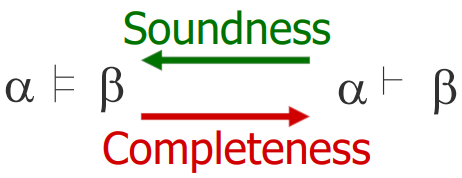
\includegraphics[width=0.3\textwidth,keepaspectratio]{soundness_completeness}
\end{figure}

\subsubsection{Monotonicity}

\begin{itemize}
\item If KB $\models \alpha$ then KB $\land \beta \models \alpha$
\item The set of entailed formulas can only increase as information is added to the KB
\item If a formula is entailed by a subset of KB, it is also entailed by KB
\end{itemize}

\newpage
\subsection{Propositional Logic}

A very simple logic (syntax, semantics, inference algorithm) centered around \textred{propositions} (statements about the world that may be true or false).

\subsubsection{Syntax}

\begin{itemize}
\item Symbols
	\begin{itemize}
	\item logical constants : True, False
	\item propositional symbols : P, Q, ...
	\item logical connectives : negation $\neg$, conjunction $\land$, disjunction $\lor$, implication $\Rightarrow$, equivalence $\Leftrightarrow$
	\item parentheses (, )
	\end{itemize}
\item Sentences
	\begin{itemize}
	\item Constructed from simple sentences
	\end{itemize}
\end{itemize}

\begin{figure}[H]
    \centering
    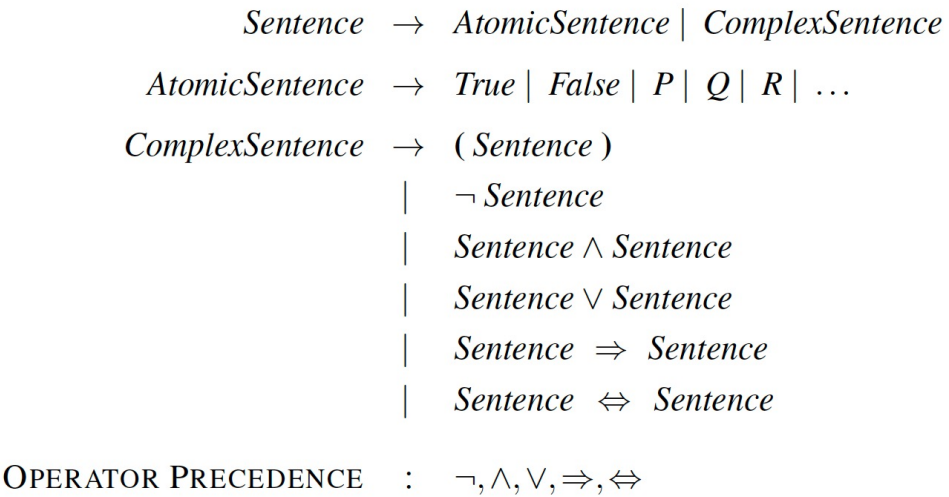
\includegraphics[width=0.6\textwidth,keepaspectratio]{syntax}
\end{figure}

\subsubsection{Model}

\begin{itemize}
\item An interpretation of a proposition formula is an assignment of a truth value to each of its proposition symbol
\item If $n$ proposition symbols : $2^n$ different interpretations 
\end{itemize}

\subsubsection{Semantics}

\begin{figure}[H]
    \centering
    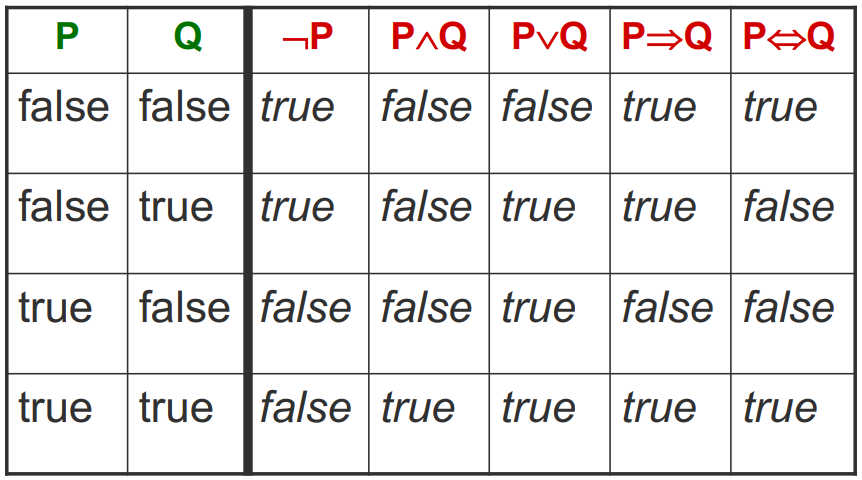
\includegraphics[width=0.5\textwidth,keepaspectratio]{truth_table}
\end{figure}

\subsubsection{Model checking}

Depth-first enumeration of all interpretations. Is is \textgreen{sound} and \textgreen{complete}.\\
For $n$ symbols :
\begin{itemize}
\item Time complexity is $\bigO (2^n)$
\item Space complexity is $\bigO (n)$
\end{itemize}

\subsection{Propositional Theorem Proving}

\subsubsection{Validity and satisfiability}

\begin{itemize}
\item \textred{Logical equivalence} : $\alpha$ and $\beta$ are logically equivalent ($\alpha \equiv \beta$) if they are true in the same interpretations ($\alpha \equiv \beta \text{ iff } \alpha \models \beta \text{ and } \beta \models \alpha$)
\item A sentence is \textred{valid} (tautology) if it is true in \textred{all} interpretations
\item A sentence is \textred{satisfiable} if it is true is \textred{some} interpretations
\item A sentence is \textred{unsatisfiable} if it is true in \textred{no} interpretations
\end{itemize}

\subsubsection{Standard Equivalences}

\begin{figure}[H]
    \centering
    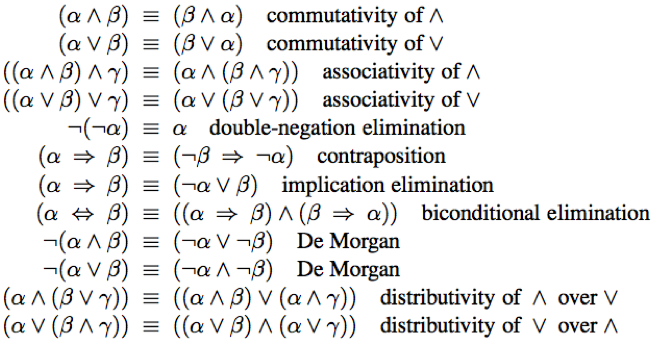
\includegraphics[width=0.6\textwidth,keepaspectratio]{standard_equivalences}
\end{figure}

\subsubsection{Proof methods}

Two kinds :
\begin{enumerate}
\item \textgreen{Application of inference rules}
	\begin{itemize}
	\item Legitimate (sound) generation of new sentences from old
	\item \textgreen{Proof} = a sequence of inference rule applications
	\item Can use inference rules as operators in a standard search algorithm
	\item Typically require transformation of sentences into a \textred{normal form}
	\end{itemize}
\item \textgreen{Model checking}
	\begin{itemize}
	\item Truth table enumeration (always exponential in $n$)
	\item Improved backtracking, e.g. : David-Putnam-Logemann-Loveland (DPLL)
	\item Heuristic search in model space (sound but incomplete), e.g. : mon-conflicts-like hill-climbing algorithms
	\end{itemize}
\end{enumerate}

\paragraph{Proof As Search}

\begin{itemize}
\item Initial state : Initial KB
\item Successor function : Each KB that results from applying one inference rule to selected rules in the KB
\item Goal test : Does the KB contain the goal sentence ?
\item Path cost : The number of inference rules applied
\end{itemize}

\subsubsection{Conjunctive Normal form (CNF)}

Every sentence in propositional logic is logically equivalent to a \textred{conjunction} of clauses (i.e. \textred{disjunction} of \textred{literals})

\paragraph{Conversion to CNF}

\begin{equation*}
B_{1,1} \Leftrightarrow (P_{1,2} \lor P_{2, 1})
\end{equation*}
\begin{itemize}
\item \textgreen{Eliminate $\Leftrightarrow$} with $(\alpha \Rightarrow \beta) \land (\beta \Rightarrow \alpha)$
	\begin{equation*}
	(B_{1,1} \Rightarrow (P_{1,2} \lor P_{2, 1})) \land ((P_{1,2} \lor P_{2, 1}) \Rightarrow B_{1,1})
	\end{equation*}
\item \textgreen{Eliminate $\Rightarrow$} with ($\neg \alpha \lor \beta$)
	\begin{equation*}
	(\neg B_{1,1} \lor (P_{1,2} \lor P_{2, 1})) \land (\neg(P_{1,2} \lor P_{2, 1}) \lor B_{1,1})
	\end{equation*}
\item \textgreen{"Move $\neg$ inwards"}, double negation, de Morgan
	\begin{equation*}
	(\neg B_{1,1} \lor P_{1,2} \lor P_{2, 1}) \land ((\neg P_{1,2} \land \neg P_{2, 1}) \lor B_{1,1})
	\end{equation*}
\item \textgreen{Distribute $\lor$ over $\land$}
	\begin{equation*}
	(\neg B_{1,1} \lor P_{1,2} \lor P_{2, 1}) \land (\neg P_{1,2} \lor B_{1, 1}) \land (\neg P_{2, 1} \lor B_{1,1})
	\end{equation*}
\end{itemize}

\subsubsection{Horn Clauses}

Linear time algorithms exist when knowledge bases are restricted to \textred{Horn clauses}. A Horn clause is a disjunction of literals of which \textgreen{at most one is positive}.

\paragraph{Inference with Horn clauses}

\begin{Parallel}[v]{0.48\textwidth}{0.48\textwidth}
\ParallelLText{
	\textred{Forward Chaining}
	\begin{itemize}
	\item Start with the knowledge base and through repeated applications of Modus Ponens, derive all logically entailed atomic sentences.
	\item Fire any rule whose premises are satisfied in the KB, add its conclusion to the KB, until query is found
	\item Data driven
	\item Sound and complete
	\end{itemize}
}
\ParallelRText{
	\textred{Backward Chaining}
	\begin{itemize}
	\item Apply resolution until empty clause if found
	\item Start with a query $q$
	\item Find all implications that conclude $q$
	\item If all premises are true, then $q$ is true, otherwise use backward chaining on premises with unknown values.
	\item Goal-directed
	\item Sound and refutation complete
	\end{itemize}
}
\ParallelPar
\end{Parallel}

\subsection{Effective Propositional Model Checking}

\subsubsection{DPLL : Davis Putman algorithm}

\begin{itemize}
\item Similar to TT-entail
\item Use a CNF input sentence
\item Recursive depth-first enumeration of interpretations
\item Various improvements (consistency, early detection of true clauses, pure symbol heuristics, unit clause heuristics)
\item One of the fastest satisfiability algorithm
\end{itemize}

\subsubsection{WalkSAT : Local Search}

\begin{itemize}
\item Model-based approach
\item Based on MinConflict CSP local search
\item Balance between greediness and randomness
\item Introduce some perturbations to avaoid local minima
\item Sound but not complete
\end{itemize}

\subsection{Summary}

\begin{figure}[H]
    \centering
    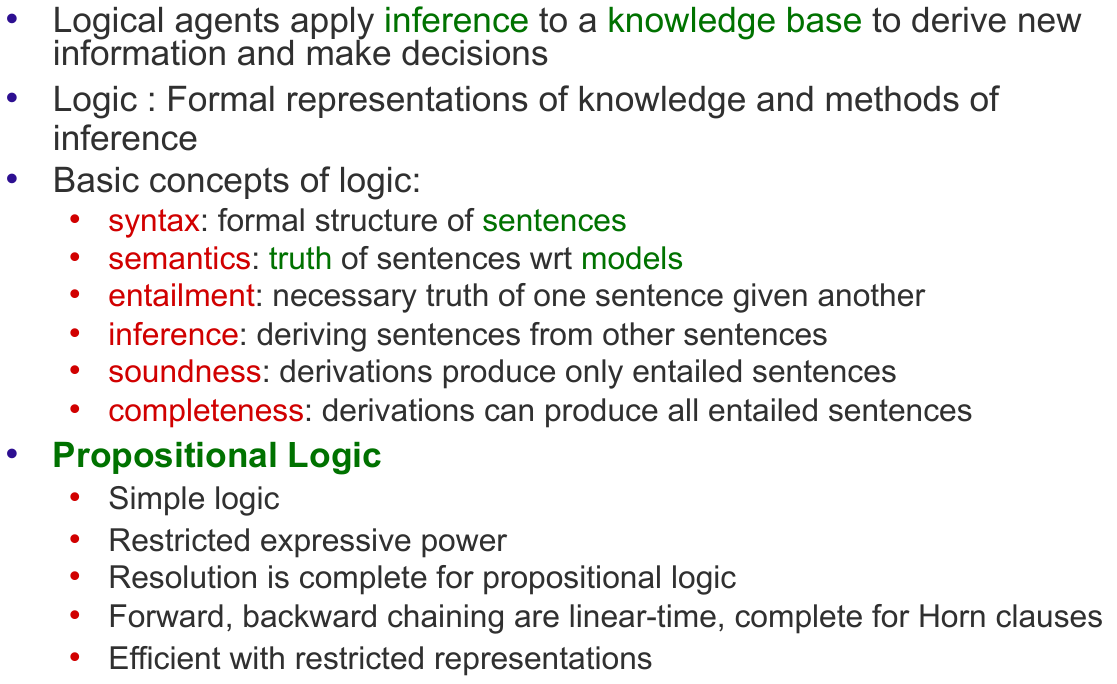
\includegraphics[width=0.5\textwidth,keepaspectratio]{summary_propositional}
\end{figure}

\section{First-Order Logic}

\subsection{Representation revisited}

\begin{itemize}
\item \textgreen{Procedural representation} : representing knowledge with data structure has limitations. Need a declarative structure.
\item \textgreen{Propositional logic} :
	\begin{itemize}
	\item Declarative : relationships between variables are described through sentences. A method for propagating relationships
	\item Expressive : can represent partial information using disjunction
	\item Compositional : if A means "it is raining" and B means "i like beer", A $\land$ B means "it is raining and I like beer"
	\item But lacks expressive power to describe the environment concisely
	\end{itemize}
\item \textgreen{FOL basic blocks}
	\begin{itemize}
	\item PL assumes the world contains \textred{facts}
	\item FOL (like natural language) assumes the world contains \textred{objects}, \textred{relations}, \textred{functions}.
	\end{itemize}
\end{itemize}

\subsection{Syntax and semantics of FOL}

\subsubsection{Syntax}

\begin{minipage}{0.52\textwidth}
	\begin{itemize}
	\item An \textred{alphabet} consists of variables, constants, function symbols, predicate symbols (all user-defined) and of connectors, punctuations and quantifiers.
	\item \textred{Terms} are either variables, constants or function symbols provided with as many terms as arguments, as the function expects
	\item \textred{Well-formed formulas} are constructed from predicate symbols, provided with terms as arguments, and from connectors, quantifiers and punctuation - according to the rules of the connectors
	\end{itemize}
\end{minipage}
\begin{minipage}{0.46\textwidth}
	\begin{figure}[H]
    		\centering
    		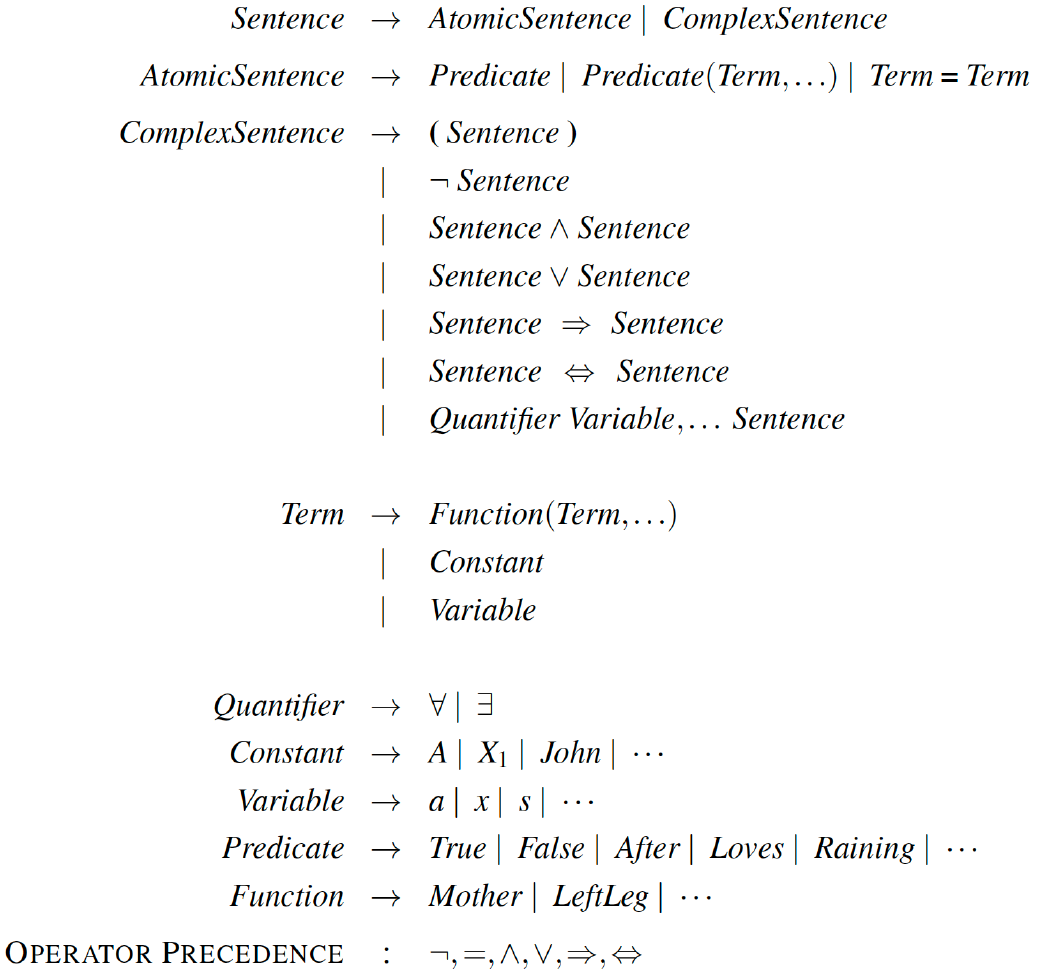
\includegraphics[width=\textwidth,keepaspectratio]{fol_syntax}
	\end{figure}
\end{minipage}

\subsubsection{Semantics}

\begin{itemize}
\item Provided by\textred{interpretations} for the basic constructs, usually suggested by meaningful names
\item \textred{Domain} of the interpretation : set of objects
\item Constants : the interpretation identifies the object in the real world
\item Predicate symbols : the interpretation specifies the particular relation in the domain. Can be defined implicitly, or explicitly through the set of tuples of objects that satisfy the relation.
\item Function symbols : identifies the object referred to by a tuple of objects. Can be defined implicitly or explicitly through tables.
\end{itemize}

\subsubsection{Interpretation}

\begin{itemize}
\item A set D (the \textred{domain})
\item A (total) function that maps constants to D
\item A (total) function that maps functions symbols to (total) functions : D $\rightarrow$ D
\item A (total) function that maps predicate symbols to predicates : D $\rightarrow$ Booleans
\end{itemize}

Usually, one has a specific interpretation in mind when writing sentences. Beware sentences can be interpreted according to any possible interpretation.

\subsubsection{Terms}

A term is a logical expression referring to an object in the interpretation.
\begin{itemize}
\item Let $I$ be an interpretation, $t_1, ..., t_n$ be terms and $f$ be a $n$-ary function symbol :
	\begin{itemize}
	\item $f(t_1, ..., t_n)$ is a term
	\item This term refers to the object $F(T_1, ..., T_n)$ in the domain $I$
		\begin{itemize}
		\item[$\rightarrow$] where $F$ is the function $D^n \rightarrow D$ associated to $f$ in $I$ and $T_1, ..., T_n$ are the interpretation of the terms $t_1, ..., t_n$ in $I$
		\end{itemize}
	\end{itemize}
\end{itemize}

\subsubsection{Atomic sentence}

An atomic sentence state a fact (true or false). It is composed of a predicate with possible arguments (terms) and is true or false in an interpretation.

\begin{itemize}
\item Let $I$ be an interpretation, $t_1, ..., t_n$ be terms and $p$ be a $n$-ary function symbol :
	\begin{itemize}
	\item $p(t_1, ..., t_n)$ is an atomic formula
	\item The formula is true if in $I$ the relation $P(T_1, ..., T_n)$ holds
		\begin{itemize}
		\item[$\rightarrow$] where $P$ is the predicate $D^n \rightarrow Boolean$ associated to $P$ in $I$ and $T_1, ..., T_n$ are the interpretation of the terms $t_1, ..., t_n$ in $I$
		\end{itemize}
	\end{itemize}
\end{itemize}

\subsubsection{Complex sentences}

A complex sentence is built by combining atomic sentences using logical connectives ($neg, \land, \lor, \Rightarrow, \Leftrightarrow$) and parentheses, and is true or false in a given interpretation.

\subsubsection{Quantifiers}

Can be used to express properties of collections of objects ($\forall, \exists$)

\paragraph{Universal quantifiers}

States that a predicate $P$ holds for all objects $x$ in the domain. Given an interpretation $I$ with domain $D$, the sentence is true if and only if all the individual sentences where the variable $x$ is replaced by the individual objects in $D$ are true in the given interpretation. Typically, $\Rightarrow$ is the main connective with $\forall$ (common mistake : using $\land$ as the main connective with $\forall$).

\paragraph{Existential quantifiers}

States that a predicate $P$ holds for some object in the universe. Given an interpretation $I$ with domain $D$, the sentence is true as there is at least one of the individual sentences where the variable $x$ is replaced by the individual objects in $D$ is true in the given interpretation. Typically, $\land$ is the main connective with $\exists$ (common mistake : using $\Rightarrow$ as the main connective with $\exists$).

\paragraph{Properties of quantifiers}

\begin{itemize}
\item \stackanchor{$\forall x \forall y$}{$\exists x \exists y$} is the same as \stackanchor{$\forall y \forall x$}{$\exists y \exists x$}
\item $\exists x \forall y$ is \textred{not} the same as $\forall y \exists x$
\end{itemize}

\paragraph{Connection between quantifiers}

\begin{itemize}
\item \stackanchor{$\forall x P$}{$\exists x P$} is equivalent as \stackanchor{$\textred{\neg} \exists x \textred{\neg} P$}{$\textred{\neg} \forall x \textred{\neg} P$}
\item This generalize : \stackanchor{$\neg (P \land Q)$}{$\neg (P \lor Q)$} equivalent to \stackanchor{$\neg P \lor \neg Q$}{$\neg P \land \neg Q$}
\end{itemize}

\subsubsection{Closed and ground formulas}

A ground term (or formula) is a term (or formula) without any variable.\\
A closed formula is a formula where each occurrence of a variable $x$ is in the scope of a quantifier $\forall x$ or $\exists x$

\subsubsection{Logical Reasoning}

An interpretation where $\alpha$ is true is called a \textred{model} of $\alpha$\\
Logical \textred{entailment} between sentence $\alpha$ and $\beta$ : $\alpha \models \beta$ if and only if, in every interpretation in which $\alpha$ is true, $\beta$ is also true.

\subsubsection{Validity and satisfiability}

\begin{itemize}
\item \textred{Validity} : a sentence that is true in \textred{all} interpretations
\item \textred{Satisfiability} : a sentence that is true is \textred{some} interpretations
\item \textred{Inconsistency, unsatisfiability} : a sentence that is \textgreen{false} is \textred{all} interpretations
\item $\alpha$ is valid iff $\neg \alpha$ is unsatisfiable
\item $\alpha \models \beta$ iff ($\alpha \neg \beta$) is unsatisfiable
\end{itemize}

\subsection{Using FOL}

FOL can be used to model natural numbers, sets and subsets, lists.

\subsection{Some complements on FOL}

\begin{itemize}
\item Completeness theorem : the set of logical consequences is recursively enumerable
\item Turing : the set of logical consequences is not recursive
\end{itemize}

\newpage
\section{Inference in FOL}

\subsection{Propositional vs. FOL interference}

How to transform FOL sentences into a propositional sentence ? Using propositional inference system.

\subsubsection{Universal instantiation}

For any sentence $\alpha$, variable $v$, and ground term $g$ : $\frac{\forall v \ \alpha}{subst({v/g}, \alpha)}$\\
A universally quantified variable can be replaced with \textgreen{any} instance. Similar to and-elimination since $\forall v \ P(v)$ is "identical" to $P(v_1) \land P(v_2) \land ... \land P(v_n)$

\subsubsection{Existential instantiation}

For any sentence $\alpha$, variable $v$, and \textred{new} constant symbol $k$ : $\frac{\exists v \ \alpha}{subst({v/k}, \alpha)}$\\
A existentially quantified variable can be replaced with a new symbol.

\subsubsection[Reduction to Propositional Logic]{Reduction to Propositional Logic (Propositionalization}

\begin{itemize}
\item Reduce FOL sentences into a set of propositional sentences.
\item Entailment is preserved
\item The set of propositional sentences is finite if no function symbol, infinite otherwise
\item Can be reduced to a finite set (for each proof)
\end{itemize}

\paragraph{Reduction (technical issues)}

\begin{itemize}
\item \textgreen{Theorem : Herbrand} : If a sentence $\alpha$ is entailed by a FOL KB, it is entailed by a \textred{finite} subset of the propositionalized KB
	\begin{itemize}
	\item \textgreen{Application} : For $n = 0$ to $\inf$ do :
		\begin{itemize}
		\item Create a propositional KB by instantiating with depth-$n$ terms
		\item See if $\alpha$ is entailed by this KB
		\end{itemize}
	\item \textgreen{Problem} : Works if $\alpha$ is entailed, loops if $\alpha$ is not entailed
	\end{itemize}
\item \textgreen{Theorem : Turing / Church} : Entailment for FOL is \textred{semidecidable} (algorithms exist that say yes to every entailed sentence, but no algorithm exists that also says no to every nonentailed sentence).
\end{itemize}

\subsection{Unification}

How to make 2 terms / atoms identical ? Find values for variables that makes the two terms identical.

Unification process : \textgreen{Unify($p,q$)}
\begin{itemize}
\item Take two atomic sentences $p$ and $q$
\item Return a substitution would make $p$ and $q$ identical
\item Unify($p,q$) $= \theta$ where Subst($\theta, p$) = Subst($\theta, q$)
\item $\theta$ is called the unifier of the two sentences, there is possibly more than one unifier.
\item Unique \textred{Most General Unifier} (up to variable renaming)
\item Quadratic complexity (size of the sentences)
\end{itemize}

\newpage
\subsubsection{Most General Unifier (mgu)}

The substitution that makes the least commitment about the binding variables. It is unique (up to variable renaming).

\paragraph{Standardize apart}

Problem if $2$ sentences share variables. Standardize apart is to renaming the variables of one or both to avoid name clashes.

\paragraph{Generalized Modus Ponens}

Let Subst($\theta, p_i$) $=$ Subst($\theta, p_i'$) for all $I$ :
\begin{equation*}
\frac{p_1', p_2', ... p_n', (p_1 \land p_2 \land ... \land p_n \Rightarrow q)}{\text{Subst}(\theta, q)}
\end{equation*} 

\subsection{Forward chaining}

\subsubsection{First Order definite clauses}

\begin{itemize}
\item Extension of propositional definite clauses
\item \textred{Definite clauses} :
	\begin{itemize}
	\item A disjunction of literals of which \textgreen{one is positive}
	\item Often written as : $A1 \land ... \land An \Rightarrow H; H\leftarrow A1, A2, ..., An$
	\item Not always possible to transform a set of FOL sentences to definite clauses
	\end{itemize}
\item Horn clauses : at most one positive literal
\end{itemize}

\subsubsection{Analysis of FC algorithm}

\begin{itemize}
\item \textgreen{Soundness} : Does it only derive sentences that are entailed ? Yes, because only (Generalized) Modus Ponens is used and it is sound
\item Does it answer every query whose answers are entailed by the KB ? Yes if the clauses are definite clauses. May not terminate in general if query is not entailed. This is unavoidable: entailment with definite clauses is semidecidable
\end{itemize}

\subsection{Backward chaining}

Start with the premises of the goal. Each premise must be supported by KB. Start with first premise and look for support from KB (looking for clauses with a head that matches premise, the head's premise must then be supported by KB).

\subsubsection{BC algorithm}

\begin{itemize}
\item FOL-BC-Ask(KB, $\alpha$)
\item Simplistic version of BC
\item A recursive, depth-first algorithm (suffers from repetition and incompleteness, space is linear)
\item Application domains : logic programming : Prolog language, and constraint programming
\end{itemize}

\newpage
\paragraph{Logic programming : Prolog}

\begin{itemize}
\item Algorithm = Logic + Control
\item basis :
	\begin{itemize}
	\item Backward chaining with horn clauses + bell \& whistles
	\item Program = set of choices
	\end{itemize}
\item Execution :
	\begin{itemize}
	\item DF, left-to-right backward chaining
	\item Built-in predicates for arithmetic etc.
	\item Built-in predicates that have side effects
	\item Closed-world assumption ("negation as failure")
	\end{itemize}
\end{itemize}

\subsubsection{And-Or Tree vs. List of goals Tree}

\begin{Parallel}[v]{0.48\textwidth}{0.48\textwidth}
\ParallelLText{
	\textred{And-Or Tree}
	\begin{itemize}
	\item Not really suitable in FOL, because of substitutions
	\item Suitable for describing forward chaining
	\item Not suitable for backward chaining : difficult to handle substitutions within and nodes
	\end{itemize}
}
\ParallelRText{
	\textred{List of goals Tree}
	\begin{itemize}
	\item Not suitable for forward chaining
	\item Suitable for backward chaining : substitutions applies on all goals in the list of goals (see algorithm FOL-BC-Ask)
	\item Resulting substitution = composition of substitutions along the successful branch
	\end{itemize}
}
\ParallelPar
\end{Parallel}

\begin{minipage}{0.475\textwidth}
  \centering
  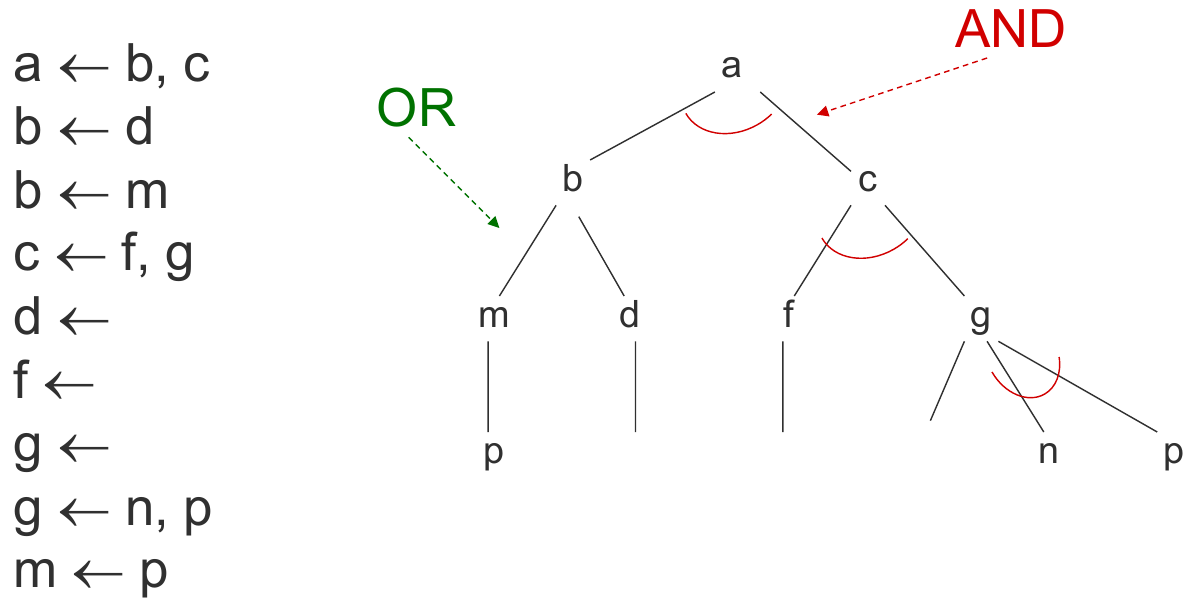
\includegraphics[width=0.8\linewidth,keepaspectratio]{and-or_tree}
\end{minipage}
\begin{minipage}{0.48\textwidth}
  \centering
  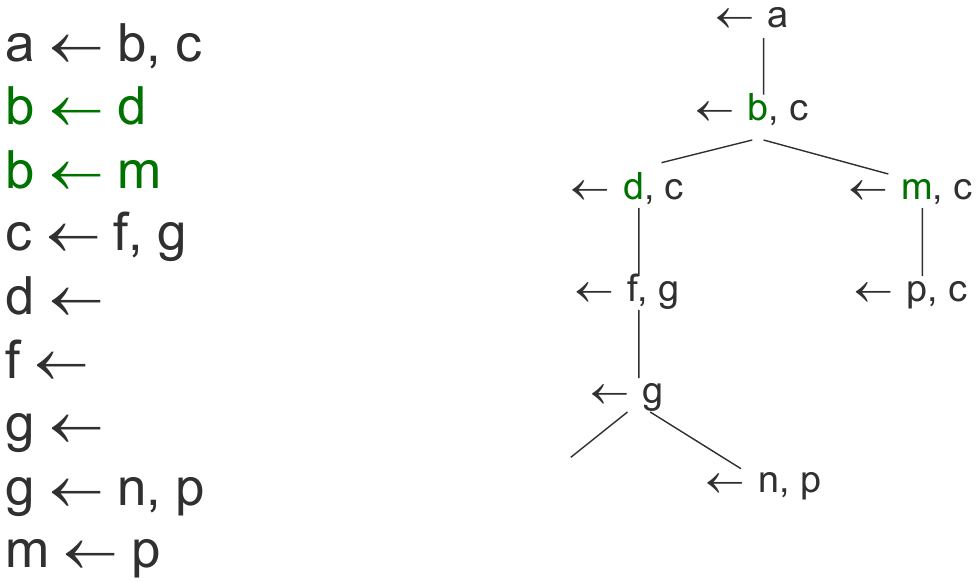
\includegraphics[width=0.8\linewidth,keepaspectratio]{list_of_goals_tree}
\end{minipage}

\subsection{Resolution}

\subsubsection{First-Order CNF}

Every sentence of first-order logic can be converted into an inferentially equivalent Conjunctive Normal Form (CNF) sentence. The two sentences are both unsatisfiable or both satisfiable.

\subsubsection{Conversion to CNF}

\begin{itemize}
\item \textbf{Eliminate implications} : Convert all implications with corresponding disjunctions
	\begin{itemize}
	\item[] $p \Rightarrow q$ becomes $\neg p \lor q$
	\end{itemize}
\item \textbf{Move $\neg$ inwards} : Use de Morgan’s laws, quantifier equivalences, and double negations
	\begin{itemize}
	\item[] $\neg (p \lor q)$ becomes $\neg p \land \neg q$
	\item[] $\neg (p \land q)$ becomes $\neg p \lor \neg q$
	\item[] $\neg \forall x, p$ becomes $\exists x \neg p$
	\item[] $\neg \exists x, p$ becomes $\forall x \neg p$
	\item[] $\neg \neg p$ becomes $p$
	\end{itemize}
\item \textbf{Standardize variables} : Change all duplicate variable names to separate names
	\begin{itemize}
	\item[] $(\forall x \ P(x)) \lor (\exists x \ Q(x))$ becomes $(\forall x \ P(x)) \lor (\exists y \ Q(y))$
	\end{itemize}
\item \textbf{Move quantifiers left} :
	\begin{itemize}
	\item[] $p \lor \forall x \ q$ becomes $\forall x \ p \lor q$
	\end{itemize}
\item \textbf{Skolemization} : Replace variables with \textred{brand new constants} (not existing elsewhere in KN) in order to remove all existential qualifiers
	\begin{itemize}
	\item[] $\forall x \ Q(x)$ becomes $Q(A)$ where A is unique
	\item \textred{Skolem Functions} are universally quantified variable sin whose scope the existential quantifier appears.
	\end{itemize}
\item \textbf{Distribute $\land$ over $\lor$} :
	\begin{itemize}
	\item[] $(a \land b) \lor c$ becomes $(a \lor c) \land (b \lor c)$
	\end{itemize}
\item \textbf{Flatten nested conjunctions and disjunctions} :
	\begin{itemize}
	\item[] $(a \lor b) \lor c$ becomes $(a \lor b \lor c)$
	\item[] $(a \land b) \land c$ becomes $(a \land b \land c)$
	\end{itemize}
\end{itemize}

\subsubsection{Resolution inference rule}

\begin{itemize}
\item Simple version :
	\begin{itemize}
	\item[] $\frac{A \land B, \neg B \land C}{A \land C}$
	\end{itemize}
\item Modus Ponens does not allow us to derive new implications, it only derives atomic conclusions.
\item Resolution : make it more powerful. Sound and complete inference system for propositional logic.
\item A lifted version of propositional resolution rule :
	\begin{itemize}
	\item Two clauses must be standardized apart (no variables are shared)
	\item Can be resolved if their literals are complementary
	\item For $p_i$ and $q_i$ where UNIFY$(p_j, \neg q_k) = \theta$ :
		\begin{itemize}
		\item[] \[\frac{{p_1 \lor ... p_j ... \lor p_m, \atop q_1 \lor ... q_k ... \lor q_n}}{\text{SUBST}(\theta \ ,(p_1 \lor ... p_{j-1} \lor p_{j+1} ... \lor p_m \lor q_1 \land ... q_{k-1} \lor q_{k+1} ... \lor q_n))}\]
		\end{itemize}
	\end{itemize}
\item How to prove that a is a logical consequence of KB (in CNF) ? 
	\begin{itemize}
	\item Proof by contradiction : KB $\models \ \alpha$ iff (KB $\land \ \neg \alpha$ unsatisfiable
	\item Transform $\neg \alpha$ into conjunctive normal form
	\item Show that KB $\land \ \neg \alpha$ is unsatisfiable (apply resolution rule until derivation of the empty clause)
	\item Possible to get an answer (substitution) that makes the goal to fail
	\end{itemize}	
\end{itemize}
